\documentclass[11pt]{article}
\usepackage[utf8]{inputenc}
\usepackage[english, ngerman]{babel}
\usepackage{amsmath,amsthm,verbatim,amssymb,amsfonts,amscd}
\usepackage{enumerate}
\usepackage{listings}
\usepackage{courier}
\usepackage[]{graphicx}
\usepackage[]{epstopdf}
\usepackage[margin=1in]{geometry}
\lstset{
  numbers=left,
  language=C,
  basicstyle=\footnotesize\ttfamily,
  breaklines=true,
  morekeywords={function, NIL}
}
\newcommand{\abs}[1]{\left| #1 \right| }
\setlength{\parindent}{0pt} 

\author{
  Felix Schrader, 3053850 \\ 
  Jens Duffert, 2843110 \\
  Eduard Sauter, 3053470
}
\title{Datenstrukturen und Algorithmen: Haus\"ubung 4}
\begin{document}
\maketitle
\subsection*{Aufgabe 2}
\begin{enumerate}[a)]
\item
In dieser Aufgabe soll der minimale Spannbaum von Punkt A durch das
Prim-Verfahren bestimmt werden. Dies wurde grafisch dargestellt. Es wurde
darauf verzichtet, alle Wege bei der Bestimmung farbig zu markieren.\\
Der Startpunkt ist A. Von A ist es möglich drei Wege zu gehen.
1.Weg zu D (Wertung 2), 2.Weg zu C (Wertung 9) und 3.Weg zu E (Wertung 9).
In der Abbildung \ref{fig:a1} links oben ist dies zu sehen.
\begin{figure}[h!]
	\centering
	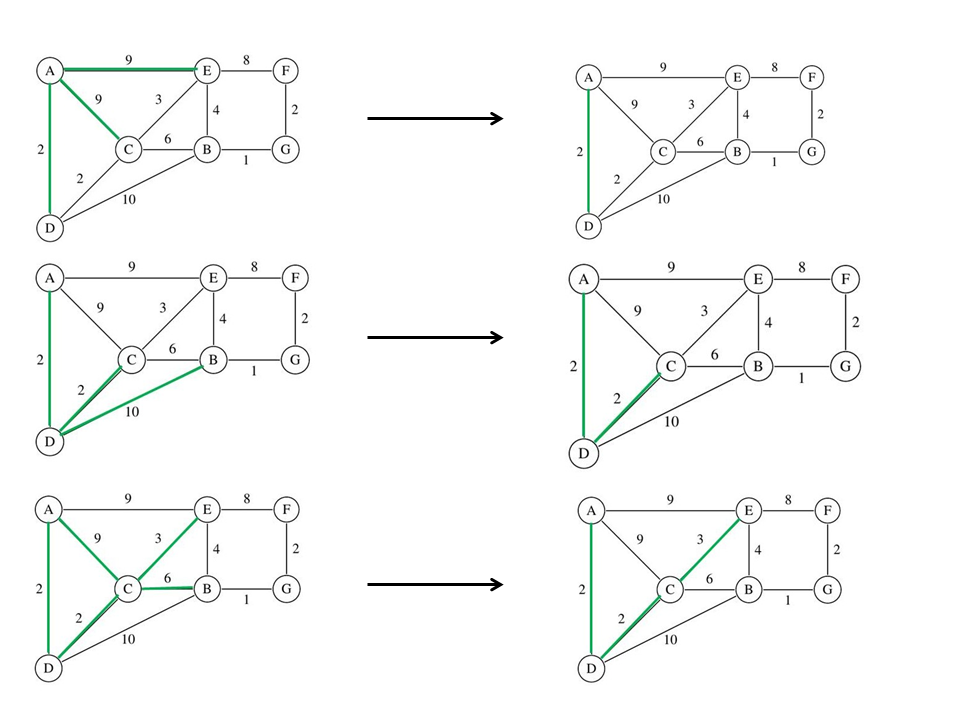
\includegraphics[width=0.8\textwidth]{aufgabe2ateil1.png}
	\caption{Grafik für Verfahren von Prim}
	\label{fig:a1}
\end{figure}
Es wird der Weg mit der geringsten Wertung genommen und somit der zu D.
Von D aus ist es möglich zu C (Wertung 2) und zu B (Wertung 10) zu gelangen.
Also sind jetzt die Wege zu E, C (je Wertung 9) und zu C (Wertung 2) und B
(Wertung 10) zur Verfügung. Auch in diesem Fall wird der Weg mit der geringsten
Wertung genommen. Dies wird mit allen weiteren Wegen gemacht.
\begin{figure}[h!]
	\centering
	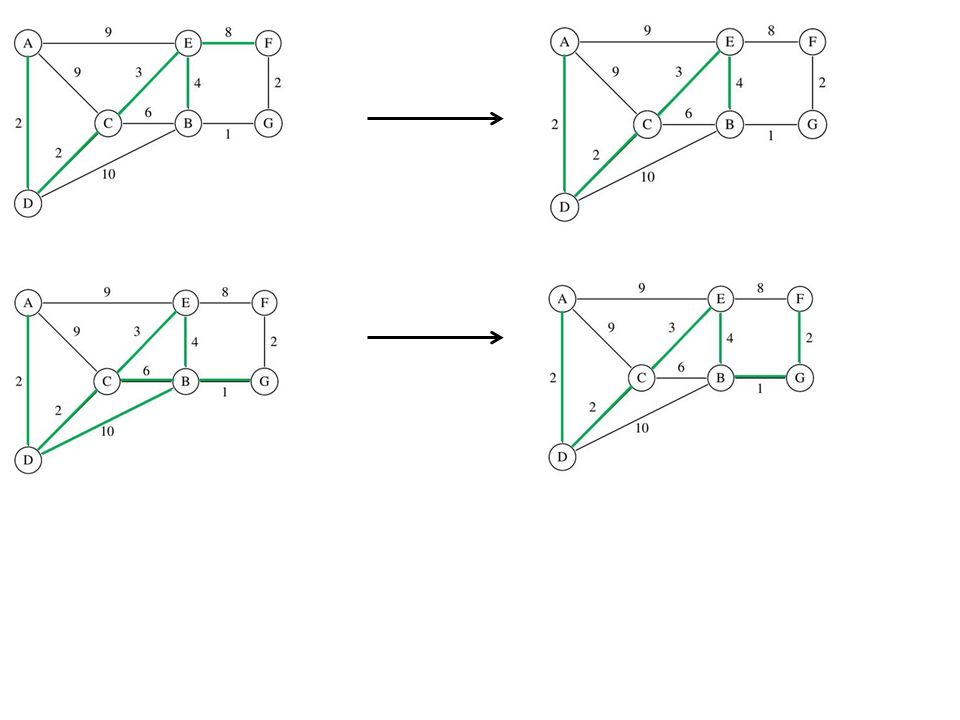
\includegraphics[width=0.8\textwidth]{aufgabe2ateil2.png}
	\caption{Grafik für Verfahren von Prim}
	\label{fig:a2}
\end{figure}
Das Ergebnis des minimalen Spannbaum ist in Abbildung \ref{fig:a2} rechts unten
zu sehen. Dieses lautet:

\begin{align*}
A \rightarrow D \rightarrow C \rightarrow E \rightarrow B \rightarrow G \rightarrow F
\end{align*}


Dieser hat einen Wert von:
\begin{align*}
2 + 2 + 3 + 4 + 1 + 2 = 17
\end{align*} 
\item
Es soll nun mit dem Dijkstra Algorithmus der kürzestes Weg von A zu F bestimmt
werden. Dabei wurden die ? in den Kästen wo noch keine Informationen vorhanden
sind weggelassen.
1.Schritt

\begin{tabular}{|c|c|c|c|c|c|c|c|c|}
	\hline  		  & A & B & C & D & E & F & G & PriorityQueue\\ 
	\hline $dist_{1}$ & 0 &   &  & 2 & 9 &	&  & $D_{2}$\\ 
	\hline $pred_{1}$ & Nil &  &  & A & A &	&  &\\
	\hline 
\end{tabular} 

2.Schritt

\begin{tabular}{|c|c|c|c|c|c|c|c|c|}
	\hline  		  & A & B & C & D & E & F & G & PriorityQueue\\ 
	\hline $dist_{1}$ & 0 & 12  & 4 & 2 & 9 &  &  & $D_{2}$\\ 
	\hline $pred_{1}$ & Nil & D & D & A & A &  &  &\\
	\hline 
\end{tabular} 

3.Schritt

\begin{tabular}{|c|c|c|c|c|c|c|c|c|}
	\hline  		  & A & B & C & D & E & F & G & PriorityQueue\\ 
	\hline $dist_{1}$ & 0 & 10  & 4 & 2 & 9 &  &  & $D_{2}$\\ 
	\hline $pred_{1}$ & Nil & C & D & A & A &  &  &\\
	\hline 
\end{tabular}  

4.Schritt

\begin{tabular}{|c|c|c|c|c|c|c|c|c|}
	\hline  		  & A & B & C & D & E & F & G & PriorityQueue\\ 
	\hline $dist_{1}$ & 0 & 10  & 4 & 2 & 7 & 15 &  & $D_{2}$\\ 
	\hline $pred_{1}$ & Nil & C & D & A & C & E &  &\\
	\hline 
\end{tabular}

Dies Ergebnis ist nicht effektiv da der kürzestes Weg 14 (Aufgabenteil a) ist und nicht 15 wie mit diesem Algorithmus


\end{enumerate}
\end{document}
